% !TEX TS-program = pdflatex
% !TEX encoding = UTF-8 Unicode

% This is a simple template for a LaTeX document using the "article" class.
% See "book", "report", "letter" for other types of document.

\documentclass[11pt]{book} % use larger type; default would be 10pt

\usepackage[utf8]{inputenc} % set input encoding (not needed with XeLaTeX)

%%% Examples of Article customizations
% These packages are optional, depending whether you want the features they provide.
% See the LaTeX Companion or other references for full information.

%%% PAGE DIMENSIONS
\usepackage{geometry} % to change the page dimensions
\geometry{a4paper} % or letterpaper (US) or a5paper or....
% \geometry{margins=2in} % for example, change the margins to 2 inches all round
% \geometry{landscape} % set up the page for landscape
%   read geometry.pdf for detailed page layout information

\usepackage{graphicx} % support the \includegraphics command and options

% \usepackage[parfill]{parskip} % Activate to begin paragraphs with an empty line rather than an indent

%%% PACKAGES
\usepackage{booktabs} % for much better looking tables
\usepackage{array} % for better arrays (eg matrices) in maths
\usepackage{paralist} % very flexible & customisable lists (eg. enumerate/itemize, etc.)
\usepackage{verbatim} % adds environment for commenting out blocks of text & for better verbatim
\usepackage{subfig} % make it possible to include more than one captioned figure/table in a single float
% These packages are all incorporated in the memoir class to one degree or another...
\usepackage{amsmath,amssymb}

%%% HEADERS & FOOTERS
\usepackage{fancyhdr} % This should be set AFTER setting up the page geometry
\pagestyle{fancy} % options: empty , plain , fancy
\renewcommand{\headrulewidth}{0pt} % customise the layout...
\lhead{}\chead{}\rhead{}
\lfoot{}\cfoot{\thepage}\rfoot{}

%%% SECTION TITLE APPEARANCE
\usepackage{sectsty}
\allsectionsfont{\sffamily\mdseries\upshape} % (See the fntguide.pdf for font help)
% (This matches ConTeXt defaults)

%%% ToC (table of contents) APPEARANCE
\usepackage[nottoc,notlof,notlot]{tocbibind} % Put the bibliography in the ToC
\usepackage[titles,subfigure]{tocloft} % Alter the style of the Table of Contents
\renewcommand{\cftsecfont}{\rmfamily\mdseries\upshape}
\renewcommand{\cftsecpagefont}{\rmfamily\mdseries\upshape} % No bold!

%%% END Article customizations

%%% The "real" document content comes below...

\title{Thesis}
\author{Fang Ni}
%\date{} % Activate to display a given date or no date (if empty),
         % otherwise the current date is printed 

\begin{document}
\maketitle

\tableofcontents

\chapter{Introduction}

\section{Pairing interaction in nuclei}

Pairing correlation plays an important role near the Fermi energy. Pairing correlation is the two-body interaction which couples two identical nucleons into $J^{\pi}=0^+$ state. There are many evidences of pairing correlation detected from experiment. The most clear evidence is shown in Fig. \ref{Sn_isotope}. All of the ground states of even-even Sn isotopes are $J^{\pi}=0^+$ states  It indicates that the ground states consist of the $J^{\pi}=0^+$ pairs is more stable than other configurations. In addition, the ground states between even-even nuclei and neighborhood odd nuclei has large gaps of binding energy. In odd nuclei, the unpaired last neutron is the last single-particle level. The odd-even mass difference  To break the $J^{\pi}=0^+$ pair, we need large energy which is about $2\Delta \approx 24A^{-1/2}$ MeV.
\begin{figure}[htbp]
 \begin{center}
    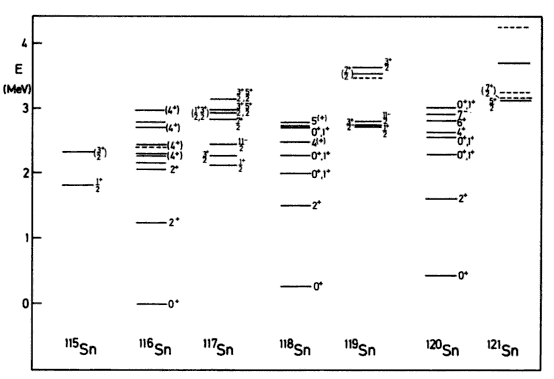
\includegraphics[width=100mm, bb=0 0 400 300]{images/Sn_isotope.png}
 \end{center}
  \caption{Low-lying excited states in Sn isotopes \cite{}. The absolute values of binding energy are adjusted at 0 MeV in the ground state of ${}^{116}$Sn.}
  \label{Sn_isotope}
\end{figure}

\subsection{A subsection}

More text.

\chapter{Pairing model}

To examine the pairing dynamics influencing the structure of nuclei, we can only concentrate the nucleons near the Fermi energy. The Hamiltonian of pairing model is
\begin{align}
	H &= \sum_l \epsilon_l n_l - g \sum_{l,l'} S_l^+ S_{l'}^- ,
\end{align}
where
\begin{align}
	n_l &= \sum_m a^{\dag}_{lm}a_{lm} \\
        S_l^{+} &= \sum_{m>0}a_{lm}^{\dag}a_{l\overline{m}}^{\dag} ,
\quad   S_l^{-} = S_l^{+\dag} 
\end{align}

\section{Exact solution}

\section{TDHFB dynamics}


\chapter{Requantization of TDHFB in integrable system}

\section{Canonical quantization}

\section{Fourier decomposition}

\section{Stationary phase to the path integral}

\section{Result}

\chapter{Requantization of TDHFB in non-integrable system}

\section{Derivation of the collective subspace in adiabatic self-consistent collective coordinate method}

\section{Application of SPA in non-integrable system}

\section{Result}

\chapter{Discussion}

\chapter{Conclusion}

\end{document}
